\chapter{Redes neuronales de propagación hacia adelante}

En este capítulo trataremos algunos de los conceptos básicos en las redes de propagación hacia adelante o en ingles \textit{feed forward neuronal networks}. Estos conceptos servirán más adelante para entender conceptos mucho más complejos. De manera abstracta, una red neuronal puede ser pensado como una función $f_{\theta}: x \to y$ tal que coge la entrada $x\in \mathbb{R}^n$ y produce una salida $y\in \mathbb{R}^m$, cuyo comportamiento está parametrizado por $\theta \in \mathbb{R}^p$, com por ejemplo $y=f_\theta(x) = \theta \cdot x$. 

\section{Unidades}

Las \textbf{unidades} (\textit{units}) son los elementos más básicos dentro de una red neuronal. Una unidad es una función que coje un valor de entrada $x\in \mathbb{R}^n$ y produce un escalar. Cada unidad está parametrizada por un peso $w \in \mathbb{R}^n$ y un término de \textit{bias} (permite al modelo desplazar la función de activación hacia la izquierda o derecha) denotado por $b$, tal que el valor de salida de cada unidad puede ser descrito como

\begin{equation}
    f\parentesis{\sum_{i=1}^n x_i \cdot w_i + b}
\end{equation}
donde $f:\mathbb{R} \to \mathbb{R}$ es lo que llamamos \textbf{función de activación}. Existe una gran cantidad de funciones de activación, y son, en general, funciones no lineales. 



\section{Estrucutra de una red neuronal}

Las unidades se organizan en \textbf{capas} (\textit{layers}), con cada capa coteniendo una o varias unidades. La última capa se le denomina \textit{capa de salida}, y todas las capas anteriores \textit{capas ocultas}. El número de unidades de una capa se le llama ancho o espesor de capa, y no todas las capas deben tener el mismo espesor, aunque las dimensiones deberán estar alineadas. El número de capas se denomina \textbf{profundidad} de la red. El \textit{input} de cada capa debe venir dado de la capa anterior excepto la primera capa, mientras que la salida de la red neuronal será el \textit{output} de la última capa. Diseñar una red neuronal implica, entre otras cosas, definir la estrucutra general de la red, incluyendo el número de capas y el ancho de las mismas.

\section{Evaluando la salida de una red neuronal}

Para cada valor de entrada $x$ (vector n-dimensional) se produce una salida computable por la red neuronal denotada por $\hat{y}$. Ahora, habrá que comparar la como de buena es la predicción de nuestra red neuronal $\hat{y}$ e $y$. Ahora es cuando entra a trabajar la función de pérdida. La \textbf{función de pérdida} mide el nivel de diferencia entre $\hat{y}$ e $y$, que denotamos por $l$. Existen decensas de funciones de pérdida en función de la tarea: clasificación binaria, multi-clasificaión, regresión... Una función de péridda típicamente compara las diferencias entre $y$ e $\hat{y}$ sobre un número de puntos mas que sobre un único punto. 

\section{Entrenando la red neuronal}

Asumiendo la misma notación, denotando por $\theta$ como el conjunto de todos los pesos y los términos \textit{bias} de todas las capas de la red. En un principio podemos suponer que $\theta$ es inicicializada con valores aleatorios, denotado por $f_{NN}$ a la función que representa la red neuronal. Con estos valores aleatorios, debemos calcular $\hat{y} = f_{NN} (x,\theta)$ y obtener $l(\hat{y},y)$. Luego tendríamos que calcular el grandiente de la función de pérdida y denotarla por $\nabla l (f_{NN}(x,\theta),y)$. El siguiente $\theta$ en ser usado será aquel calculado como $\theta_s=\theta_{s-1} - \alpha \cdot l (f_{NN}(x,\theta),y)$, siendo $\alpha$ un parámetro libre que podremos seleccionar en función de valores anteriores. Luego el $\theta$ final será aquel que nos de un valor razonalbe de $l(\hat{y},y)$. 

\section{Derivando funciones coste usando Maxima Verosimilitud}

En esta sección nos centraremos en como derivar las funciones pérdida usando el método de Máxima Verosimilitud. Especificamente, veremos como noralmente usamos las funciones pérdidas en el aprendizaje profundo, con la entropía cruzada binaria, entropía cruzada y error cuadrático. 

La idea de la Máxima Verosimilitud es intentar obtener el $\theta$ que maximiza una función, en general suele ser la probabilidad $P(D|\theta)$ siendo esto la \textit{probabilida de que ocurra D condicionado a $\theta$}. Una vez fijado $\theta$, vemos que probabilidad hay de obtener los datos $D$. Lógicamente el mejor $\theta$ será el que sea capaz de reproducir los datos $D$, que es lo que viene a decir ``maximizar $P(D|\theta)''$. En función del problema planteado, de la forma de los datos $D$, pues tendremos una forma de $P(D|\theta)$ u otra. 

\subsection{Entropía binaria cruzada}

La Entropía Binaria Cruzada viene dada por la siguiente expresión: 

\begin{equation}
    - \sum_{i=1}^{n} y_i \log f (x_i,\theta) + (1-y_i) \log (1-f(x_i,\theta))
\end{equation}
es la mejor función de pérdida cuando hablamos de clasificación binaria. Es usada cuando la red neuronal se usa para predecir la probabilidad de un resultado. En algunos casos, la capa de salida tiene una sola unidad con una función sigmoide apropiada como función de activación. 


\subsection{Entropía cruzada}

La entropía cruzada viene dada por la expresión 

\begin{equation}
    - \sum_{i=1}^n y_i \log f(x_i,\theta)
\end{equation}
es la función recomendada para la función de pérdida para la multi-clasficación. Esta función de pérdidad debería de trabajar, a priori, para predecir la probabilidad de determinados resultados de cada una de las clases. En muchos casos, la capa de salida tiene unidades \textit{softmax}.

\subsection{Error cuadrático}

El error cuadrático viene dado por la expresión

\begin{equation}
    \sum_{i=1}^{i} (y-\hat{y})^2
\end{equation}
y se suele usar para problemas de regresión. La capa de salida tiene una única undiad. 

\section{Tipos de Unidades/Capas/Funciones de Activación}

Las propiedes de las funciones de activación más comunes:

\begin{itemize}
    \item En teoría, cuando una función de activación es no lineal, una capa de dos redes neuronales puede \textit{aproximar cualquier función} (siempre y cuando se le de un número adecuados entre las capas ocultas). Por eso quereos funciones no lineales en general.
    \item Una función de activación debería ser continuamente diferencialbe, lo que permitirá al gradiente ser calculado y poder usar métodos basados en el gradiente, lo que nos permitirá encontrar los parámetros que minimicen la función error sobre los datos. 
    \item Una función con rango finito lleva a una activiada mucho más estable. 
    \item Las funciones suaves son preferidas (por razones puramente empíricas).
    \item Deberían ser simétricas respecto al origen y comportarse como función identidad cerca del mismo $f(x)=x$. 
\end{itemize}

\subsection{Unidad Lineal}

La unidad lineal es la unidad más simple, ya que transforma el \textit{input} tal que $y=w x + b$. Tal y como indica el nombre, la unidad es lineal, y se suele usar para generar la media de una distribución gausiana. Las unidades lineales hacen que el aprendizaje basado en gradientes sea una tarea bastante sencilla.

\subsection{Unidad Sigmoide}

\begin{minipage}{0.45\linewidth}
    La Unidad Sigmoide da el siguiente valor de salida a partir de la entrada

    \begin{equation}
        y = \frac{1}{1+e^{-(w x + b)}}
    \end{equation}
    siendola función de activación

    \begin{equation}
        f(x) = \frac{1}{1+e^{-x}}
    \end{equation}
    Las unidades sigmoides pueen ser usadas en las capas de salida junto con la entropía binaria cruzada para problemas de clasificación binaria. La salida de esta unidad puede ser modelada como una función de Bernoulli sobre la $y$ condicionada a $x$. 
\end{minipage} \hfill
\begin{minipage}{0.52\linewidth}
    \centering
    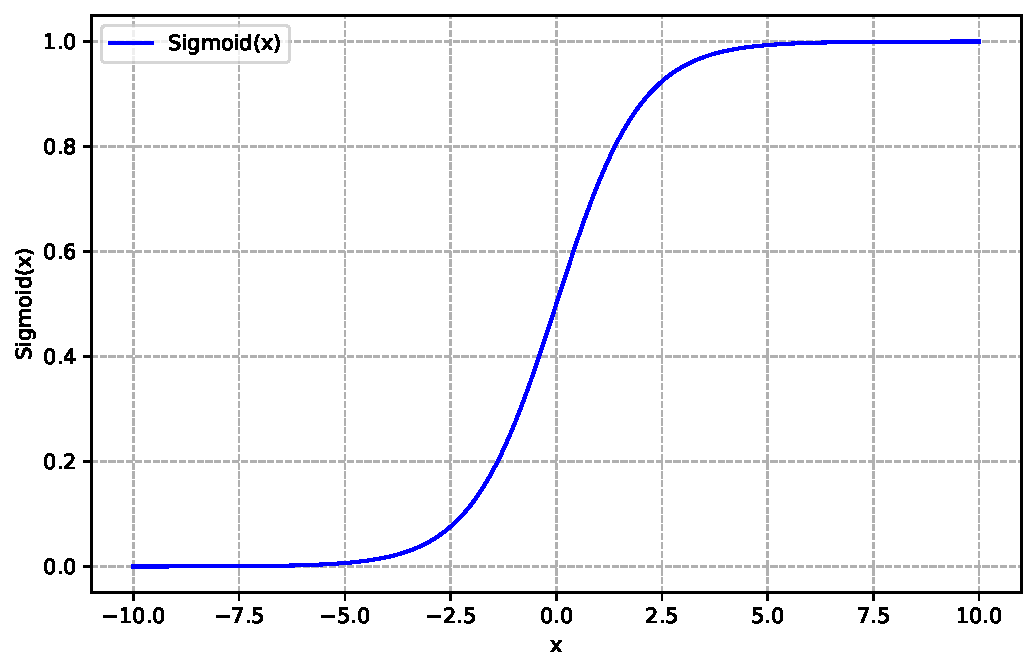
\includegraphics[width=1\linewidth]{Imagenes/03/Sigmoide.pdf}
    \captionof{figure}{Función sigmoide.}
\end{minipage}

\subsection{Capa \textit{Softmax}}

Las capas \textit{Softmax} (\textit{Softmax layers}) se usa típicamente como una capa de salida para tareas de multi-clasificación junto con la función error Entropía Cruzada. Su función es normalizar las salidas de las capas anteriores de tal modo que todas sumen uno. Normalmente, las unidades de capas anteriores nos darán un valor no normalizado acerca de como el valor de entrada se relaciona o depende con determinada clásica. La capa softmax normalizada lo que hace es, efectivamente, dar el valor de probabilidad de cada clase. 



\subsection{ReLU} 
\begin{minipage}{0.45\linewidth} 

La \textit{Rectified Linear Unit} (Unidad Lineal Rectificada) usada junto con la función de transformación lineal, usa la siguiente función de activación

\begin{equation}
    f(x) = \max (0,\omega x + b),
\end{equation}
Es usada en general como capa oculta. Se puede probar que las unidades ReLU dan gradientes muy consistentes, lo que mejora los métodos basados en estos.

\end{minipage} \hfill
\begin{minipage}{0.52\linewidth}
    \centering
    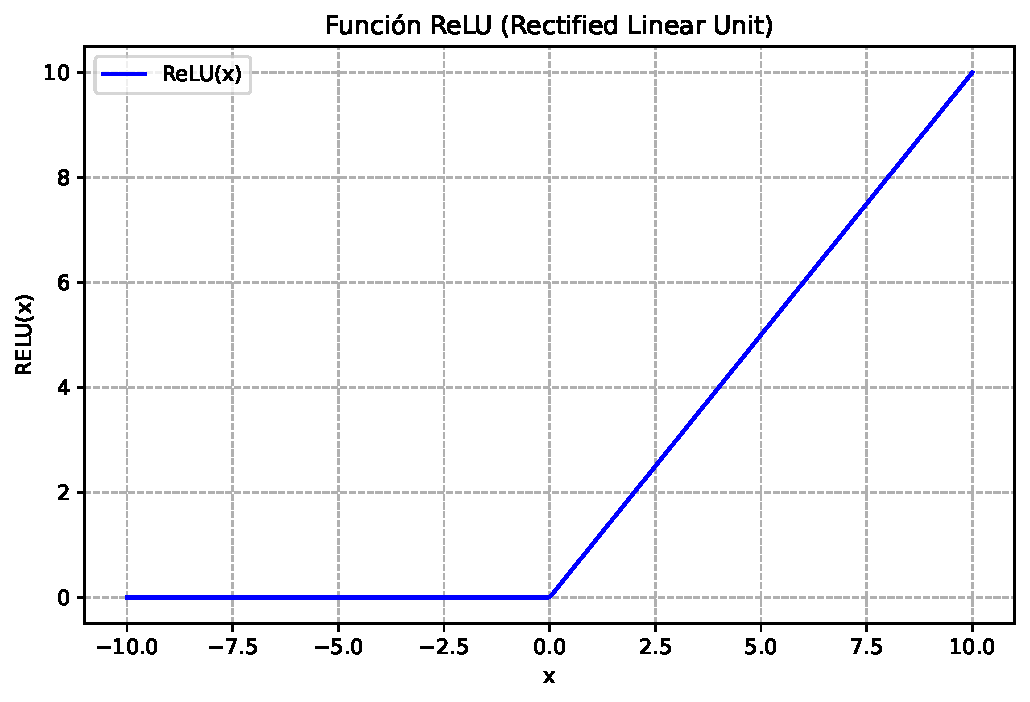
\includegraphics[width=1\linewidth]{Imagenes/03/ReLU.pdf}
    \captionof{figure}{Función sigmoide.}
\end{minipage}


\subsection{Tangente Hiperbólica}

\begin{minipage}{0.45\linewidth} 

    La tangente hiperbólica trnaforma el \textit{input} tal y como sigue: 

    \begin{equation}
        y = \tanh (\omega x + b)
    \end{equation}
    siendo claramente la función de activacióin

    \begin{equation}
        f(x) = \tanh (x)
    \end{equation}
    Se suele unidad como capa/unidad oculta, y en conjunción con la función de transoformación lineal. 

\end{minipage} \hfill
\begin{minipage}{0.52\linewidth}
    \centering
    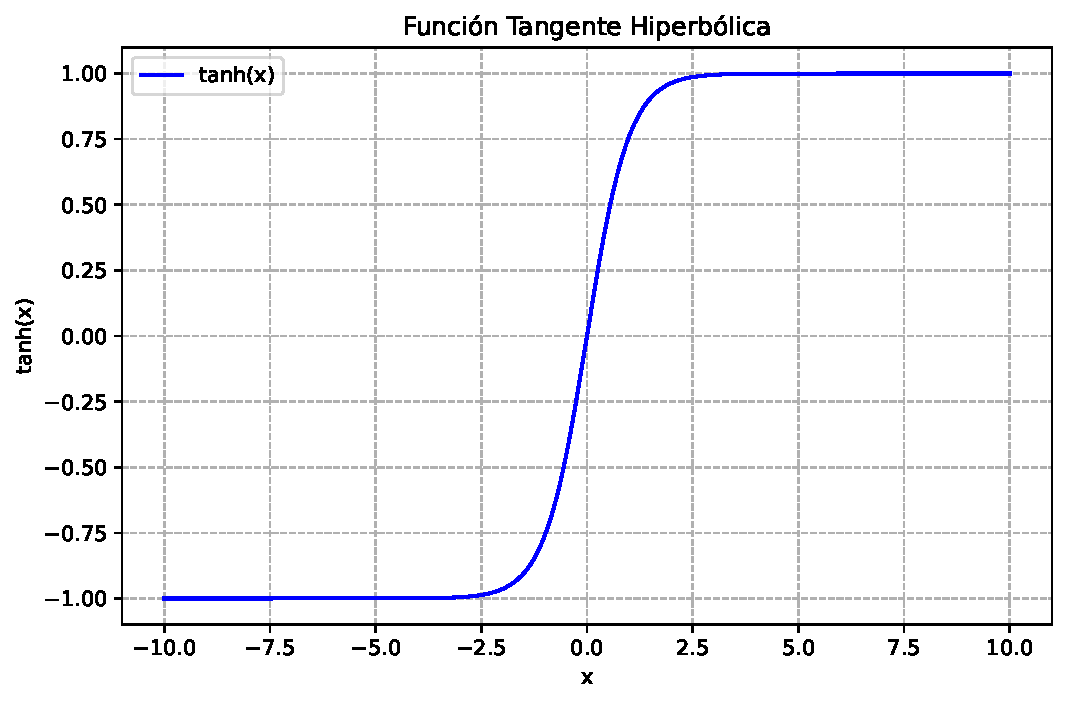
\includegraphics[width=1\linewidth]{Imagenes/03/Tanh.pdf}
    \captionof{figure}{Función sigmoide.}
\end{minipage}


